\documentclass[11pt, oneside,table]{article}   	% use "amsart" instead of "article" for AMSLaTeX format
%\usepackage{geometry}                		% See geometry.pdf to learn the layout options. There are lots.
\usepackage[margin=.7in]{geometry}
\geometry{letterpaper}                   		% ... or a4paper or a5paper or ... 
%\geometry{landscape}                		% Activate for for rotated page geometry
\usepackage[parfill]{parskip}    		% Activate to begin paragraphs with an empty line rather than an indent
\usepackage{graphicx}				% Use pdf, png, jpg, or eps� with pdflatex; use eps in DVI mode
\usepackage{moreverb}						% TeX will automatically convert eps --> pdf in pdflatex		
\usepackage{amssymb}
\usepackage{mathtools}
\usepackage[framed,numbered,]{mcode}
\usepackage{listings}
\usepackage{xcolor}
\usepackage{amsmath}
\lstset { %
    backgroundcolor=\color{black!7}, % set backgroundcolor
    basicstyle=\footnotesize,% basic font setting
}

\newcommand{\bigo}{$\mathcal{O}$}

\title{MATH 6644\\Homework 1}
\author{Stephan Boettcher}
%\date{}                                           % Activate to display a given date or no date

\begin{document}
\maketitle
\section*{Question 1}
{\it Construct a dense 3$\times$3 matrix G with $\rho$(G)$>$1. Define an iteration and find an example of $\vec{x}_0$ and $\vec{c}$ such that the iteration does not converge.} \newline
Beginning with the dense A matrix of: $
A = \begin{bmatrix}
1& 2& 1          \\[0.3em]
4& 9           & 2 \\[0.3em]
     7           & 20 &2
     \end{bmatrix}
  $ , we generate the G matrix by first constructing the N and M matrices. The M matrix is defined as the diagonal elements of A and the N matrix is defined as: N=M-A, or the off diagonal elements multiplied by -1. The G matrix is then constructed by $G=M^-1*N$, which creates the following matrix:
$
G = \begin{bmatrix}
0 & -2& -1          \\[0.3em]
       -\frac{4}{9} & 0           & -\frac{2}{9} \\[0.3em]
       \frac{7}{2}           & -10& 0
     \end{bmatrix}
  $ .  The spectral radius of the G matrix is 2.9413. This spectral radius makes for an unstable iteration matrix that will most likely result in the iterative method going to infinity, rather than converging on a value. An iteration for this matrix is defined as: 
  $$ \vec{x}_{k+1}=G\vec{x}_k+\vec{c}
  $$
Where $\vec{c}$ is defined as: $\vec{c}=M^{-1}\vec{b}$. The $\vec{b}$ is the final vector we are iterating to. To find an $\vec{x}_0$,$\vec{c}_0$, the vector $\vec{b}$ must be defined. For this assignment, the following values were chosen for these vectors:
\newline
{\begin{center}
$\vec{b} = \begin{bmatrix}
3          \\[0.3em]
4 \\[0.3em]
5
     \end{bmatrix}
  $  ,  $\vec{x}_0 = \begin{bmatrix}
1          \\[0.3em]
0 \\[0.3em]
1
     \end{bmatrix}
  $  ,  $\vec{c}_0 = \begin{bmatrix}
0          \\[0.3em]
1 \\[0.3em]
0
     \end{bmatrix}
  $ 
  \end{center}
With these values, combined with the unstable G matrix, the iterative method quickly spirals out of control and goes to infinity within 100 iterations. 

%%%%%%%%%%%%%%%%%%%%%%%%%%%%%%%%%%%%%%%%%%%%%%%%%%%%%%%%
\section*{Question 2}
{\it Give the matrix expression for the symmetric Gauss-Seidel iterations.}\newline
The Gauss-Seidel (G-S) method can be expressed as both an element-wise expression and in matrix expressions. To express the G-S method in matrix expression form, the notation must first be developed. Given an n$\times$n  nonsingular matrix A, $\vec{x}\in  \mathbb{R}^n$, and $\vec{b}\in    \mathbb{R}^n$, we can split the A matrix into:
$$ A=D-E-F$$
where D is the diagonal elements of A, E is the lower triangular matrix of A, and F is the upper triangular matrix of A. With these matrices defined, the symmetric G-S iteration can be expressed in matrix form. 

The symmetric G-S requires two sweeps: a forward sweep followed by a backward sweep. This is done to increase the rate of convergence of the G-S method. The forward sweep portion of the iteration is defined as:
$$ \vec{x}^{k+\frac{1}{2}}=(D-E)^{-1}F\vec{x}^{\ (k)}+(D-F)^{-1}\vec{b}$$
The forward sweep is then followed by the backward sweep which is defined as:
$$ \vec{x}^{k+1}=(D-F)^{-1}E\vec{x}^{\ (k+\frac{1}{2})}+(D-F)^{-1}\vec{b}$$

Thus, the matrix expression for the symmetric G-S iterations is:
\begin{align*}
\vec{x}^{k+\frac{1}{2}}=(D-E)^{-1}F\vec{x}^{\ (k)}+(D-F)^{-1}\vec{b} \\
\vec{x}^{k+1}=(D-F)^{-1}E\vec{x}^{\ (k+\frac{1}{2})}+(D-F)^{-1}\vec{b}
\end{align*}

%%%%%%%%%%%%%%%%%%%%%%%%%%%%%%%%%%%%%%%%%%%%%%%%%%%%%%%%
\section*{Question 3}
{\it Assume A is a n$\times$n symmetric positive definite matrix with all eigenvalues in the intervals (1; 1.1) $\cup$ (10; 10.2). Assume that the cost of a matrix vector multiplication is about 4$n$ floating point multiplications. Estimate the number of floating point operations reduce the A-norm of the error by a factor of $10^{-3}$ using CG iterations.}\newline

Because the n$\times$n A matrix is symmetric positive definite, convergence can be guaranteed for the Conjugate Gradient(CG) method. This allows an upper limit on the number of floating point operations (FLOPS) to be calculated. This upper bound will be dependent on the theoretical convergence rate of the CG method. The analysis of the CG method assumes that variable assignment and vector addition/subtraction can occur in \bigo(1) or constant time. This is theoretically possible on vector machines. The analysis also assumes that 'vector devision' (i.e. the computation of the $\alpha$ and $\beta$ values) can also be completed in \bigo(4n). The breakdown of the FLOPS cost per step of the CG method is below:


\begin{align*}
\vec{r}^{\ (0)} &= \vec{b}-A\vec{x}  &   4n\ FLOPS \\
 \vec{p}^(0)&= \vec{r}^{\ (0)} &   1\ FLOPS\\
for\ i &= 1:k\ & k\ iterations \\
\{\\
\vec{q}^{\ (k-1)}&=A\vec{p}^{\ (k-1)} & 4n\ FLOPS \\
\alpha_{k-1}&=\frac{<\vec{r}^{\ (k-1)},\vec{r}^{\ (k-1)}>}{<\vec{p}^{\ (k-1)},\vec{q}>} & 8n\ FLOPS\ total \\
\vec{x}^{\ (k)} &= \vec{x}^{\ (k-1)} + \alpha_{k-1}\vec{p}^{\ (k-1)} &  4n\ FLOPS\\
\vec{r}^{\ (k)} &= \vec{r}^{\ (k-1)} - \alpha_{k-1}\vec{q} &  4n\ FLOPS\\
\beta_{k-1}&=\frac{<\vec{r}^{\ (k)},\vec{r}^{\ (k)}>}{<\vec{r}^{\ (k-1)},\vec{r}^{\ (k-1)}>} & 8n\ FLOPS\ total \\
\vec{p}^{\ (k)} &= \vec{r}^{\ (k)} + \beta_{k-1}\vec{p}^{\ (k-1)} &  4n\ FLOPS\\
\}
\end{align*}

Thus it takes \bigo(36n) FLOPS to complete one iteration. The error equation is given by:
$$ ||\vec{e}^{\ (k+1)}||_A \le \Bigg(\frac{\sqrt{\kappa(A)}-1}{\sqrt{\kappa(A)}+1}\Bigg)||\vec{e}^{\ (k)}||_A
$$
For this problem, $\kappa(A)=\frac{10.2}{1.1}= 9.\overline{2727}$. By the error equation above, for each iteration, the error will be reduced by $\Bigg(\frac{\sqrt{9.\overline{2727}}-1}{\sqrt{9.\overline{2727}}+1}\Bigg)\approx 0.5056$. As a result, after 10 iterations, the error will be reduced by $\approx 10^{-3}$. Thus, the number of FLOPS to reduce the A-norm of the error by a factor of $10^{-3}$ is \bigo(360n).
%%%%%%%%%%%%%%%%%%%%%%%%%%%%%%%%%%%%%%%%%%%%%%%%%%%%%%%%
\section*{Question 4}
{\it Assume that A is a n$\times$n symmetric positive definite matrix. If $\kappa$(A) =\bigo(n), give a rough estimate of the number of CG iterations required to reduce the relative residual to \bigo($\frac{1}{n}$). }\newline

The residual matrix is defined as $\vec{r}^{\ (k)}=\vec{b}-A\vec{x}^{\ (k)}$. The error vector can be written as $A\vec{e}^{\ (k)} =A(\vec{x}^{\ (*)} -\vec{x}^{\ (k)} )=\vec{b}-A\vec{x}^{\ (k)}$. Thus, $\vec{r}^{\ (k)}=A\vec{e}^{\ (k)} $. Since $\kappa$(A) =\bigo(n), the error equation can be written as:

$$ ||A^{-1}\vec{r}^{\ (k+1)}||_A \le \Bigg(\frac{\sqrt{\mathcal{O}(n)}-1}{\sqrt{\mathcal{O}(n)}+1}\Bigg)||A^{-1}\vec{r}^{\ (k)}||_A
$$

To determine the number of iterations necessary to reduce the error to a given value, the following equation must be solved:
$$\Bigg(\frac{\sqrt{\mathcal{O}(n)}-1}{\sqrt{\mathcal{O}(n)}+1}\Bigg)^x=\mathcal{O}\Big(\frac{1}{n}\Big)
$$
where x is the number of iterations. Solving for x, we get:

$$x=\frac{-log(\mathcal{O}(n))}{log(\sqrt{\mathcal{O}(n)}-1)-log(\sqrt{\mathcal{O}(n)}+1)}
$$

To provide a quicker, rougher estimate, the above equation follows the equation $x'=\frac{3*2^{log(n)}}{4}$ fairly closely for multiple values of $n$. While the values provided by $x'$ do not exactly match that generated by $x$, the $x'$ values can be computed quicker and will give the correct order of magnitude. 
%%%%%%%%%%%%%%%%%%%%%%%%%%%%%%%%%%%%%%%%%%%%%%%%%%%%%%%%
\section*{Question 5}
{\it Discreteize the following differential equation:
$$\begin{cases} -u'' +4u = & x\in [0,1] \\ u(0)=-1, & u(1)=2 \end{cases}
$$

by the central difference scheme. Write your linear system of equations (you must give the matrix A and $\vec{b}$). Solve the system by using classical iteration such as Jacobi, Gauss-Seidel and SOR with n = 1000. Test you relaxation parameter in SOR for several values and decide which one is better. You need to discuss your results.}\newline

The above differential equation can be solved analytically to generate a truth curve, against which the numerical methods can be compared. The solution for this particular ODE is:
$$u(x)=\frac{e^{-2x}(e^{4x}+2e^{4x+2}-2e^2-e^4)}{e^4-1}
$$

To solve this equation numerically, the equation must first be discretized via the central difference theorem. The first step is to discretize the term $-u''$:
$$u''=\frac{d^2u}{dx^2}=\frac{1}{h}\Bigg(\frac{u(x+h)-u(x)}{h}-\frac{u(x)-u(x-h)}{h}\Bigg) = \frac{1}{h^2}\bigg(u(x+h)-2u(x)+u(x-h)\bigg)
$$

This gives the final form of the differential equation, with the same boundary conditions, of:
$$0=-\frac{1}{h^2}\bigg(u(x+h)-2u(x)+u(x-h)\bigg)+4u(x)
$$
Realizing that $h=x_i-x_{i-1}$, this can be simplified and rewritten as:
$$0=u_{i+1}-2u_i+u_{i-1}-4h^2u_i
$$

This form of the equation can be used to generate the A and $\vec{b}$ variables, where $A\vec{u}=\vec{b}$:

{\begin{center}
$A= \begin{bmatrix}
-2-4h^2 & 1 &0 &0 &0&\dots&0          \\[0.3em]
1 &-2-4h^2 & 1 &0 &0&\dots&0     \\[0.3em]
0 &1 &-2-4h^2 & 1 &0 &\dots&0 \\[0.3em]
&&\ddots &\ddots &\ddots \\[0.3em]
0&\dots&\dots&\dots&\dots&1&-2-4h^2 
     \end{bmatrix}
  $  ,  $\vec{u} = \begin{bmatrix}
u_1          \\[0.3em]
u_2\\[0.3em]
\vdots \\[0.3em]
u_{n-2}\\[0.3em]
u_{n-1}
     \end{bmatrix}
  $  ,  $\vec{b}= \begin{bmatrix}
1          \\[0.3em]
0 \\[0.3em]
\vdots\\[0.3em]
0\\[0.3em]
-2
     \end{bmatrix}
  $ 
  \end{center}

where $h=\frac{1}{n}$. This discretized ODE was then solved using the Gauss-Jacobi , Gauss-Seidel, and SOR with $n=1000$. 

The A matrix as well as the b and u vectors were created with the following code:
\lstinputlisting{SetupProb5.m}

The first algorithm tested was the Gauss-Jacobi method. This is the simplest algorithm to implement and has a simple iteration. The G-J method is computed by the equation: 
$$x_i^{(k+1)}=\frac{1}{a_{ii}}\bigg(b_i+\sum\limits_{\substack{j=1\\ j\ne i}}^n a_{ij}x_j^{(k)}\bigg) \ \ \ \ \ \ \ \ i=1:n
$$
The G-J algorithm can quickly be implemented in just a few lines in Matlab, using Matlab's vector notation. The implementation used for this problem is shown below.
\lstinputlisting{Jacobi.m}
The G-J method was run with a number of different convergence criteria to demonstrate the convergence properties of this method. Figure \ref{gj} shows these convergence values.

\begin{figure}[!h]
\begin{center}
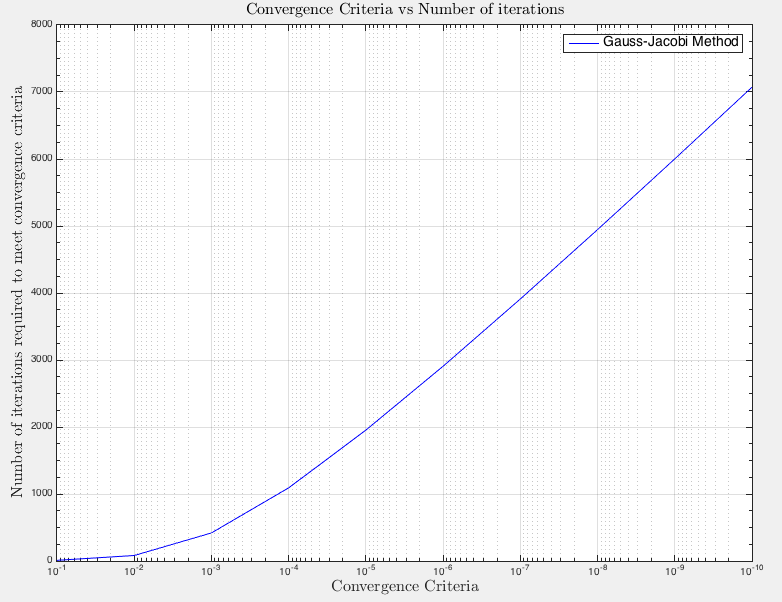
\includegraphics[width=130mm]{gj.png}
\caption{Convergence of the G-J method.}
\label{gj}
\end{center}
\end{figure}

The second algoritm implemented was the Gauss-Seidel method. The G-S method splits the A matrix into the D, E, and F subparts. The D matrix contains all of the diagonal elements of A. The E and F matrices are the upper and lower triangular matrices, respectively, of A. The G-S algorithm then computes the following iteration:

$$ \vec{x}^{\ (k+1)}=(D-E)^{-1}F\vec{x}^{\ (k)}+(D-F)^{-1}\vec{b}
$$
The G-S algorithm can also be quite quickly implemented in just a few lines in Matlab, using Matlab's vector notation. Notably, precomputing the values of $(D-E)^{-1}F$ and $(D-F)^{-1}\vec{b}$ greatly speedup the runtime of the algorithm, as these values are invariant. The implementation used for this problem is shown below.
\lstinputlisting{GS.m}

The G-S method was run with a number of different convergence criteria to demonstrate the convergence properties of this method. Figure \ref{gs} shows these convergence values. The chart also compares the relative performance of the G-J and G-S methods. As can be seen, the G-S method 

\begin{figure}[!h]
\begin{center}
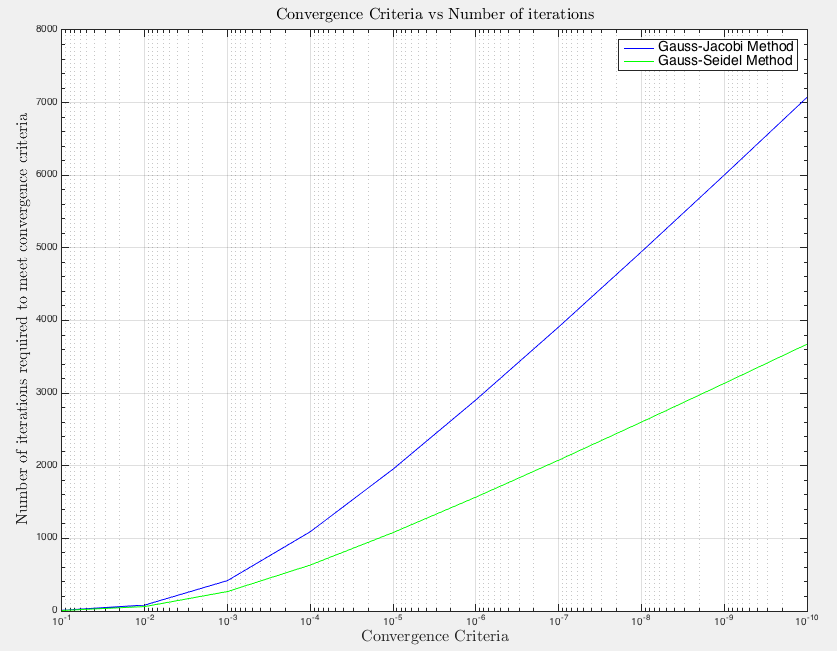
\includegraphics[width=130mm]{gs.png}
\caption{Convergence of the G-S method compared to the G-J method.}
\label{gs}
\end{center}
\end{figure}

%\begin{figure}[htbp]
%\begin{center}
%\begin{tabular}{ | l | c|c| c| c | c | c| c| c| c  | c | }
%\hline
%  &A & B & C &D &E&F&G&H&I&J\ \\\hline
%  Design1 &240 & 350 & 305 & 30 & 35& 400& 90& 0& 30& 300 \\\hline
%% Design2 &300 & 380 & 370 & 34 & 40& 400& 100& 50& 100& 100 \\\hline
%%  Design3 &300 & 600 & 580 & 40 & 50& 550& 100& 150& 200& 250 \\\hline
%
%\end{tabular}
%\caption{Design 1 Parameters}
%\end{center}
%\end{figure}
%
%The isometric view of this design can be seen in Figure \ref{d1i}. The large cylinder was plotted using multiple instances of the \mcode{surf} command on two cylinders. Figure \ref{d1y} and Figure \ref{d1z} show the printer design in the X-Y and X-Z plains, respectively.
%
%\begin{figure}[htbp]
%\begin{center}
%\includegraphics[width=160mm]{d1iso.png}
%\caption{An isometric view of Design 1}
%\label{d1i}
%\end{center}
%\end{figure}



\end{document}  